\subsection{Nekonečně hluboká pravoúhlá jáma se schodem}   
Částice o hmotnosti $M$ se pohybuje v potenciálu
\begin{equation}
    V(x)=\left\{\begin{array}{ll} \infty & x<0 \\ V_{0} & 0<x<\frac{a}{2} \\ 0 & \frac{a}{2}<x<a \\ \infty & x>a\end{array}\right.
\end{equation}
viz obrázek~\ref{fig:WKBStep}.
Nalezněte WKB vlnovou funkci a spektrum pro $E>V_{0}$.

\begin{figure}[!htbp]
	\centering
		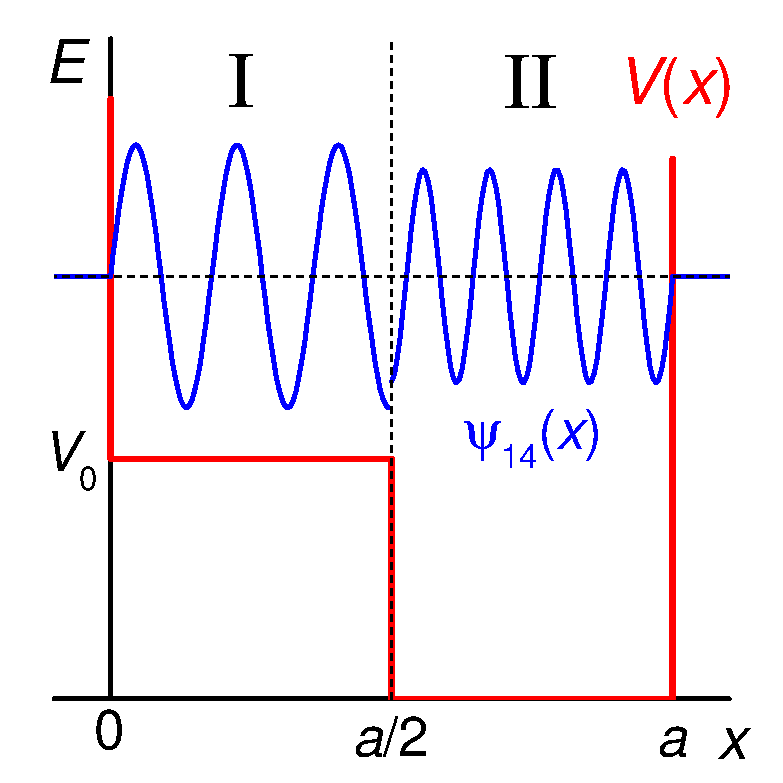
\epsfig{file=schod.eps,width=0.4\linewidth,keepaspectratio}
		\scaption{
			Nekonečně hluboká pravoúhlá jáma se schodem.
			Potenciál červeně.
			Modře zobrazena 14. vlnová funkce pro hodnoty parametrů $a=V_{0}=2$, $M=1$, $\hbar=0.1$.
			Příslušná energie je $E_{14}=3,52$.
		}
	\label{fig:WKBStep}
\end{figure}		
	
\begin{solution}
	Kinematicky dostupné oblasti označíme
	\begin{align}
		\text{I:} & \quad 0<x<\frac{a}{2}\,, \nonumber\\
		\text{II:} & \quad \frac{a}{2}<x<a\,.\nonumber
	\end{align}
	Klasická hybnost v těchto oblastech pak je
    \begin{subequations}
        \begin{align}
            p_{\mathrm{I}}&=\sqrt{2M\left(E-V_{0}\right)},\\
            p_{\mathrm{II}}&=\sqrt{2ME}
        \end{align}            
    \end{subequations}
	(hybnost je v uvedených intervalech konstantní, nezávisí na souřadnici).
	Zintegrování v mezích $(0,x)$ dá akci
    \begin{subequations}
        \begin{align}
            S_{\mathrm{I}}(x)&=\int_{0}^{x}p_{\mathrm{I}}\d x'=xp_{\mathrm{I}},\\
            S_{\mathrm{II}}(x)
                &=\int_{0}^{\frac{a}{2}}p_{\mathrm{I}}\d x'+\int_{\frac{a}{2}}^{x}p_{\mathrm{II}}\d x'=\frac{a}{2}p_{\mathrm{I}}+\left(x-\frac{a}{2}\right)p_{\mathrm{II}}.
        \end{align}            
    \end{subequations}
	Vlnová funkce tedy je
    \begin{subequations}
        \begin{align}
            \psi_{\mathrm{I}}(x)&=\frac{1}{\sqrt{\abs{p_{\mathrm{I}}}}}\left[C\sin{\frac{S_{\mathrm{I}}(x)}{\hbar}}+D\cos{\frac{S_{\mathrm{I}}(x)}{\hbar}}\right],\\
            \psi_{\mathrm{II}}(x)&=\frac{1}{\sqrt{\abs{p_{\mathrm{II}}}}}\left[C\sin{\frac{S_{\mathrm{II}}(x)}{\hbar}}+D\cos{\frac{S_{\mathrm{II}}(x)}{\hbar}}\right]
        \end{align}            
    \end{subequations}
	(komplexní exponenciály byly rozepsány pomocí funkcí $\sin$, $\cos$).
	Díky tomu, že se obě akce počítají od stejného počátečního bodu $x_{0}=0$, jsou konstanty $C,D$ pro vlnové funkce v obou oblastech stejné.
	
	V dalším kroku se aplikují okrajové podmínky:
	\begin{subequations}
		\begin{align}
			\psi_{\mathrm{I}}(0)&=0 && \Longrightarrow & D&=0,\\
			\psi_{\mathrm{II}}(a)&=0 && \Longrightarrow & \sin{\frac{S_{\mathrm{II}}(x)}{\hbar}}&=0.
		\end{align}			
	\end{subequations}
	Z druhé rovnice vyplývá postupně
	\begin{align}
		S_{\mathrm{II}}(x)&=\pi n\nonumber\\
		\frac{a}{2\hbar}\left[\sqrt{2M(E-V_{0})}+\sqrt{2ME}\right]&=\pi n\nonumber\\
		E-\frac{V_{0}}{2}+\sqrt{E(E-V_{0})}&=2\underbrace{\frac{\pi^{2}\hbar^{2}n^{2}}{2Ma^{2}}}_{E_{n}^{(0)}}\nonumber\\
		E_{n}^{(0)}-E+\frac{V_{0}}{2}&=\sqrt{E(E-V_{0})}\nonumber\\
		E_{n}\equiv E&=E_{n}^{(0)}+\frac{V_{0}}{2}+\frac{V_{0}^{2}}{16E_{n}^{(0)}}\,,
		\label{eq:WKBStepEnergy}
	\end{align}
	kde $E_{n}^{(0)}$, $n\in\mathbb{N}$ označuje $n$-tou hladinu nekonečně hluboké pravoúhlé jámy.
	Pro energie dostatečně vysoko nad $V_{0}$ vymizí poslední člen, což znamená, že částice se pohybuje, jako kdyby se schod rozprostřel po celé šířce jámy a dno jámy se tak zvedlo o $V_{0}/2$.

	Explicitně vyjádřená vlnová funkce je
	\begin{subequations}
		\begin{align}
			\psi_{\mathrm{I},n}(x)&=\frac{c}{\sqrt[4]{2M\left(E_{n}-V_{0}\right)}}\sin{\left\{\frac{\sqrt{2M\left(E_{n}-V_{0}\right)}}{\hbar}x\right\}},\\
			\psi_{\mathrm{II},n}(x)&=\frac{c}{\sqrt[4]{2ME_{n}}}\sin{\left\{\frac{\sqrt{2M\left(E_{n}-V_{0}\right)}}{\hbar}\frac{a}{2}+\frac{\sqrt{2ME_{n}}}{\hbar}\left(x-\frac{1}{2}\right)\right\}}\,,
		\end{align}			
	\end{subequations}
	kde energie jsou dány vzorcem~\eqref{eq:WKBStepEnergy}.
	
	WKB vlnová funkce \emph{není spojitá} v bodě $x=\frac{a}{2}$, což je patrné z příkladu na obrázku~\ref{fig:WKBStep}.
\end{solution}
